\documentclass[journal,12pt,twocolumn]{IEEEtran}
%
\usepackage{setspace}
\usepackage{gensymb}
\usepackage{xcolor}
\usepackage{caption}
%\usepackage{subcaption}
%\doublespacing
\singlespacing

%\usepackage{graphicx}
%\usepackage{amssymb}
%\usepackage{relsize}
\usepackage[cmex10]{amsmath}
\usepackage{mathtools}
%\usepackage{amsthm}
%\interdisplaylinepenalty=2500
%\savesymbol{iint}
%\usepackage{txfonts}
%\restoresymbol{TXF}{iint}
%\usepackage{wasysym}
\usepackage{hyperref}
\usepackage{amsthm}
\usepackage{mathrsfs}
\usepackage{txfonts}
\usepackage{stfloats}
\usepackage{cite}
\usepackage{cases}
\usepackage{subfig}
%\usepackage{xtab}
\usepackage{longtable}
\usepackage{multirow}
%\usepackage{algorithm}
%\usepackage{algpseudocode}
%\usepackage{enumerate}-get 
\usepackage{enumitem}
\usepackage{mathtools}
%\usepackage{iithtlc}
%\usepackage[framemethod=tikz]{mdframed}
\usepackage{listings}
\usepackage{polynom}


%\usepackage{stmaryrd}


%\usepackage{wasysym}
%\newcounter{MYtempeqncnt}
\DeclareMathOperator*{\Res}{Res}
%\renewcommand{\baselinestretch}{2}
\renewcommand\thesection{\arabic{section}}
\renewcommand\thesubsection{\thesection.\arabic{subsection}}
\renewcommand\thesubsubsection{\thesubsection.\arabic{subsubsection}}

\renewcommand\thesectiondis{\arabic{section}}
\renewcommand\thesubsectiondis{\thesectiondis.\arabic{subsection}}
\renewcommand\thesubsubsectiondis{\thesubsectiondis.\arabic{subsubsection}}

%\renewcommand{\labelenumi}{\textbf{\theenumi}}
%\renewcommand{\theenumi}{P.\arabic{enumi}}

% correct bad hyphenation here
\hyphenation{op-tical net-works semi-conduc-tor}

\lstset{
language=Python,
frame=single, 
breaklines=true,
columns=fullflexible
}



\begin{document}
%

\theoremstyle{definition}
\newtheorem{theorem}{Theorem}[section]
\newtheorem{problem}{Problem}
\newtheorem{proposition}{Proposition}[section]
\newtheorem{lemma}{Lemma}[section]
\newtheorem{corollary}[theorem]{Corollary}
\newtheorem{example}{Example}[section]
\newtheorem{definition}{Definition}[section]
%\newtheorem{algorithm}{Algorithm}[section]
%\newtheorem{cor}{Corollary}
\newcommand{\BEQA}{\begin{eqnarray}}
\newcommand{\EEQA}{\end{eqnarray}}
\newcommand{\define}{\stackrel{\triangle}{=}}
\bibliographystyle{IEEEtran}
%\bibliographystyle{ieeetr}
\providecommand{\nCr}[2]{\,^{#1}C_{#2}} % nCr
\providecommand{\nPr}[2]{\,^{#1}P_{#2}} % nPr
\providecommand{\mbf}{\mathbf}
\providecommand{\pr}[1]{\ensuremath{\Pr\left(#1\right)}}
\providecommand{\qfunc}[1]{\ensuremath{Q\left(#1\right)}}
\providecommand{\sbrak}[1]{\ensuremath{{}\left[#1\right]}}
\providecommand{\lsbrak}[1]{\ensuremath{{}\left[#1\right.}}
\providecommand{\rsbrak}[1]{\ensuremath{{}\left.#1\right]}}
\providecommand{\brak}[1]{\ensuremath{\left(#1\right)}}
\providecommand{\lbrak}[1]{\ensuremath{\left(#1\right.}}
\providecommand{\rbrak}[1]{\ensuremath{\left.#1\right)}}
\providecommand{\cbrak}[1]{\ensuremath{\left\{#1\right\}}}
\providecommand{\lcbrak}[1]{\ensuremath{\left\{#1\right.}}
\providecommand{\rcbrak}[1]{\ensuremath{\left.#1\right\}}}
\theoremstyle{remark}
\newtheorem{rem}{Remark}
\newcommand{\sgn}{\mathop{\mathrm{sgn}}}
\providecommand{\abs}[1]{\left\vert#1\right\vert}
\providecommand{\res}[1]{\Res\displaylimits_{#1}} 
\providecommand{\norm}[1]{\lVert#1\rVert}
\providecommand{\mtx}[1]{\mathbf{#1}}
\providecommand{\mean}[1]{E\left[ #1 \right]}
\providecommand{\fourier}{\overset{\mathcal{F}}{ \rightleftharpoons}}
\providecommand{\ztrans}{\overset{\mathcal{Z}}{ \rightleftharpoons}}
%\providecommand{\hilbert}{\overset{\mathcal{H}}{ \rightleftharpoons}}
\providecommand{\system}{\overset{\mathcal{H}}{ \longleftrightarrow}}
	%\newcommand{\solution}[2]{\textbf{Solution:}{#1}}
\newcommand{\solution}{\noindent \textbf{Solution: }}
\providecommand{\dec}[2]{\ensuremath{\overset{#1}{\underset{#2}{\gtrless}}}}
\numberwithin{equation}{section}
%\numberwithin{equation}{subsection}
%\numberwithin{problem}{subsection}
%\numberwithin{definition}{subsection}
\newcommand{\myvec}[1]{\ensuremath{\begin{pmatrix}#1\end{pmatrix}}}
\newcommand{\mydet}[1]{\ensuremath{\begin{vmatrix}#1\end{vmatrix}}}
\makeatletter
\def\pld@CF@loop#1+{%
    \ifx\relax#1\else
        \begingroup
          \pld@AccuSetX11%
          \def\pld@frac{{}{}}\let\pld@symbols\@empty\let\pld@vars\@empty
          \pld@false
          #1%
          \let\pld@temp\@empty
          \pld@AccuIfOne{}{\pld@AccuGet\pld@temp
                            \edef\pld@temp{\noexpand\pld@R\pld@temp}}%
           \pld@if \pld@Extend\pld@temp{\expandafter\pld@F\pld@frac}\fi
           \expandafter\pld@CF@loop@\pld@symbols\relax\@empty
           \expandafter\pld@CF@loop@\pld@vars\relax\@empty
           \ifx\@empty\pld@temp
               \def\pld@temp{\pld@R11}%
           \fi
          \global\let\@gtempa\pld@temp
        \endgroup
        \ifx\@empty\@gtempa\else
            \pld@ExtendPoly\pld@tempoly\@gtempa
        \fi
        \expandafter\pld@CF@loop
    \fi}
\def\pld@CMAddToTempoly{%
    \pld@AccuGet\pld@temp\edef\pld@temp{\noexpand\pld@R\pld@temp}%
    \pld@CondenseMonomials\pld@false\pld@symbols
    \ifx\pld@symbols\@empty \else
        \pld@ExtendPoly\pld@temp\pld@symbols
    \fi
    \ifx\pld@temp\@empty \else
        \pld@if
            \expandafter\pld@IfSum\expandafter{\pld@temp}%
               {\expandafter\def\expandafter\pld@temp\expandafter
                    {\expandafter\pld@F\expandafter{\pld@temp}{}}}%
                {}%
        \fi
        \pld@ExtendPoly\pld@tempoly\pld@temp
        \pld@Extend\pld@tempoly{\pld@monom}%
    \fi}            
\@addtoreset{figure}{problem}
\makeatother
\lstset{
language=Python,
frame=single, 
breaklines=true,
columns=fullflexible
}
\let\StandardTheFigure\thefigure
%\renewcommand{\thefigure}{\theproblem.\arabic{figure}}
\renewcommand{\thefigure}{\theproblem}
%\numberwithin{figure}{subsection}
\def\putbox#1#2#3{\makebox[0in][l]{\makebox[#1][l]{}\raisebox{\baselineskip}[0in][0in]{\raisebox{#2}[0in][0in]{#3}}}}
     \def\rightbox#1{\makebox[0in][r]{#1}}
     \def\centbox#1{\makebox[0in]{#1}}
     \def\topbox#1{\raisebox{-\baselineskip}[0in][0in]{#1}}
     \def\midbox#1{\raisebox{-0.5\baselineskip}[0in][0in]{#1}}
\vspace{3cm}
\title{ 
%\logo{
Digital Signal Processing
%}
%	\logo{Octave for Math Computing }
}
\author{AI21BTECH11017 \\ Akshitha Kola} 
\maketitle
%\newpage
\tableofcontents
%\renewcommand{\thefigure}{\thesection.\theenumi}
%\renewcommand{\thetable}{\thesection.\theenumi}
\renewcommand{\thefigure}{\theenumi}
\renewcommand{\thetable}{\theenumi}
\renewcommand{\vec}{\textbf}
%\renewcommand{\theequation}{\thesection}
\bigskip

\begin{abstract}
This manual provides a simple introduction to digital signal processing.
\end{abstract}

\section{Software Installation}
Run the following commands
\begin{lstlisting}
sudo apt-get update
sudo apt-get install libffi-dev libsndfile1 python3-scipy  python3-numpy python3-matplotlib 
sudo pip install cffi pysoundfile 
\end{lstlisting}

\section{Digital Filter}
\begin{enumerate}[label=\thesection.\arabic*
,ref=\thesection.\theenumi]
\item
\label{prob:input}
Download the sound file from  
\begin{lstlisting}
	https://github.com/AkshithaKola/EE3900/blob/main/filter/code/Sound%20Noise.wav
\end{lstlisting}


\item
\label{prob:spectrogram}
You will find a spectrogram at \href{https://academo.org/demos/spectrum-analyzer}{\url{https://academo.org/demos/spectrum-analyzer}}. 
Upload the sound file that you downloaded in Problem \ref{prob:input} in the spectrogram  and play.  Observe the spectrogram. What do you find?\\
\solution There are a lot of yellow lines between 440 Hz to 5.1 KHz.  These represent the synthesizer key tones. Also, the key strokes
are audible along with background noise.

\item
\label{prob:output}
Write the python code for removal of out of band noise and execute the code.
\\
\solution The following is the python code to remove band noise
\begin{lstlisting}
	https://github.com/AkshithaKola/EE3900/blob/main/filter/code/2.3.py
\end{lstlisting}

\item
The output of the python script in Problem \ref{prob:output} is the audio file Sound\_With\_ReducedNoise.wav. Play the file in the spectrogram in Problem \ref{prob:spectrogram}. What do you observe?
\\
\solution The key strokes as well as background noise is subdued in the audio.  Also,  the signal is blank for frequencies above 5.1 kHz.\\
The reduced noise audio file is
\begin{lstlisting}
	https://github.com/AkshithaKola/EE3900/blob/main/filter/code/Sound%20With%20ReducedNoise.wav
\end{lstlisting}
\end{enumerate}

\section{Difference Equation}
\begin{enumerate}[label=\thesection.\arabic*,ref=\thesection.\theenumi]
\item Let
\label{def:xn}
\begin{equation}
x(n) = \cbrak{\underset{\uparrow}{1},2,3,4,2,1}
\end{equation}
Sketch $x(n)$.\\
\solution 
\begin{lstlisting}
	https://github.com/AkshithaKola/EE3900/blob/main/filter/code/3.2.py
\end{lstlisting}
\item Let
\begin{multline}
\label{eq:iir_filter}
y(n) + \frac{1}{2}y(n-1) = x(n) + x(n-2), 
\\
 y(n) = 0, n < 0
\end{multline}
Sketch $y(n)$.
\\
\solution The following code yields Fig. \ref{fig2}
\begin{figure}[!ht]
\begin{center}
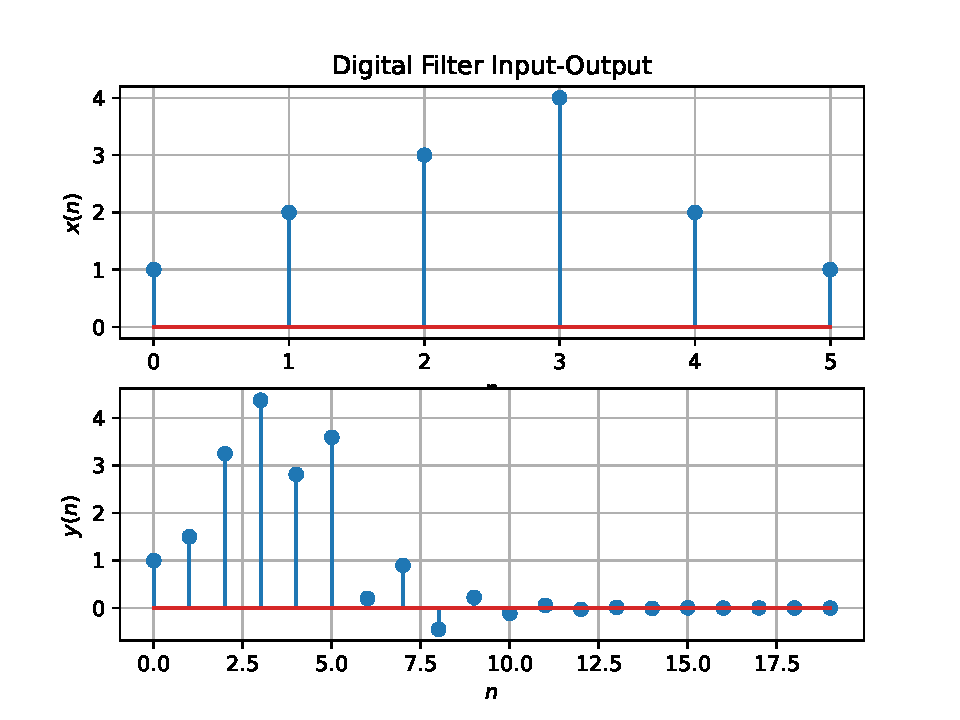
\includegraphics[width=\columnwidth]{3.2.pdf}
\end{center}
\captionof{figure}{}
\label{fig2}	
\end{figure}
\end{enumerate}

\section{Z-transform}
\begin{enumerate}[label=\thesection.\arabic*,ref=\thesection.\theenumi]
\item The $Z$-transform of $x(n)$ is defined as
%
\begin{equation}
\label{eq:z_trans}
X(z)={\mathcal {Z}}\{x(n)\}=\sum _{n=-\infty }^{\infty }x(n)z^{-n}
\end{equation}
%
Show that
\begin{equation}
\label{eq:shift1}
{\mathcal {Z}}\{x(n-1)\} = z^{-1}X(z)
\end{equation}
and find
\begin{equation}
	{\mathcal {Z}}\{x(n-k)\} 
\end{equation}
\solution From \eqref{eq:z_trans},
\begin{align}
{\mathcal {Z}}\{x(n-k)\} &=\sum _{n=-\infty }^{\infty }x(n-1)z^{-n}
\\
&=\sum _{n=-\infty }^{\infty }x(n)z^{-n-1} = z^{-1}\sum _{n=-\infty }^{\infty }x(n)z^{-n}
\end{align}
resulting in \eqref{eq:shift1}. Similarly, it can be shown that
%
\begin{equation}
\label{eq:z_trans_shift}
	{\mathcal {Z}}\{x(n-k)\} = z^{-k}X(z)
\end{equation}

\item Obtain $X(z)$ for $x(n)$ defined in problem \ref{def:xn}.\\
\solution
\begin{align}
	X(z)={\mathcal{Z}}\{x(n)\} &= \sum_{n=-\infty}
^{\infty}x(n)z^{-n}\\ &= 1+2z^{-1}+3z^{-2}+4z^{-3}+2z^{-4}+z^{-5}
\end{align}	
\item Find
%
\begin{equation}
H(z) = \frac{Y(z)}{X(z)}
\end{equation}
%
from  \eqref{eq:iir_filter} assuming that the $Z$-transform is a linear operation.
\\
\solution  Applying \eqref{eq:z_trans_shift} in \eqref{eq:iir_filter},
\begin{align}
Y(z) + \frac{1}{2}z^{-1}Y(z) &= X(z)+z^{-2}X(z)
\\
\implies \frac{Y(z)}{X(z)} &= \frac{1 + z^{-2}}{1 + \frac{1}{2}z^{-1}}
\label{eq:freq_resp}
\end{align}

\item Find the Z transform of 
\begin{equation}
\delta(n)
=
\begin{cases}
1 & n = 0
\\
0 & \text{otherwise}
\end{cases}
\end{equation}
and show that the $Z$-transform of
\begin{equation}
\label{eq:unit_step}
u(n)
=
\begin{cases}
1 & n \ge 0
\\
0 & \text{otherwise}
\end{cases}
\end{equation}
is
\begin{equation}
U(z) = \frac{1}{1-z^{-1}}, \quad \abs{z} > 1
\end{equation}
\solution It is easy to show that
\begin{equation}
\delta(n) \ztrans 1
\end{equation}
and from \eqref{eq:unit_step},
\begin{align}
U(z) &= \sum _{n= 0}^{\infty}z^{-n}
\\
&=\frac{1}{1-z^{-1}}, \quad \abs{z} > 1
\end{align}
using the formula for the sum of an infinite geometric progression.

\item Show that 
\begin{equation}
\label{eq:anun}
a^nu(n) \ztrans \frac{1}{1-az^{-1}} \quad \abs{z} > \abs{a}
\end{equation}
\solution Let $a^nu(n) = v(n)$
\begin{align}
     V(z) &= \sum _{n= 0}^{\infty}a^nu(n)z^{-n}\\
     &= \sum _{n= 0}^{\infty}a^nz^{-n}\\
     &= \sum _{n= 0}^{\infty}(az^{-1})^{n}\\
     &= \frac{1}{1-az^{-1}} 
\end{align}
%
\item 
Let
\begin{equation}
   H\brak{e^{\j \omega}} = H\brak{z = e^{\j \omega}}.
\end{equation}
Plot $\abs{H\brak{e^{\j \omega}}}$.  Comment.  $H(e^{\j \omega})$ is
known as the {\em Discret Time Fourier Transform} (DTFT) of $x(n)$.
\\
\solution The following code plots Fig. \ref{fig:dtft}.
\begin{lstlisting}
	https://github.com/AkshithaKola/EE3900/blob/main/filter/code/4.5.py
\end{lstlisting}

Using \eqref{eq:freq_resp}, we observe that $\left|H\brak{e^{\j\omega}}\right|$ is given by
\begin{align}
	\left|H\brak{e^{\j\omega}}\right| &= \left|\frac{1 + e^{-2\j\omega}}{1 + \frac{1}{2}e^{-\j\omega}}\right| \\
									  &= \sqrt{\frac{\brak{1 + \cos{2\omega}}^2 + \brak{\sin{2\omega}}^2}{\brak{1 + \frac{1}{2}\cos{\omega}}^2 + \brak{\frac{1}{2}\sin{\omega}}^2}}\\
									  &= \sqrt{\frac{2\brak{1 + \cos{2\omega}}}{\frac{5}{4} + \cos{\omega}}} \\
									  &= \sqrt{\frac{2\brak{2\cos^2{\omega}}}{\frac{5}{4} + \cos{\omega}}} \\
									  &= \frac{4|\cos{\omega}|}{\sqrt{5 + 4\cos{\omega}}}
\end{align}
The period of numerator is $\pi$ and the period of denominator is 2$\pi$\\
$\therefore$The period of $\left|H\brak{e^{\j\omega}}\right|$ is LCM($\pi$,2$\pi$)
\begin{align}
	\left|H\brak{e^{\j\brak{\omega + 2\pi}}}\right| &=\frac{4\abs{\cos\brak{\omega + 2\pi}}}{\sqrt{5+4\cos\brak{\omega +2\pi}}} \\
	&= \frac{4\abs{\cos{\omega}}}{\sqrt{5+4\cos{\omega}}}\\
	\abs{H\brak{e^{\j\brak{\omega+2\pi}}}} &= \abs{H\brak{e^{\j\omega}}}
\end{align}
and so its fundamental period is $2\pi$.
\begin{figure}[!ht]
     \centering
     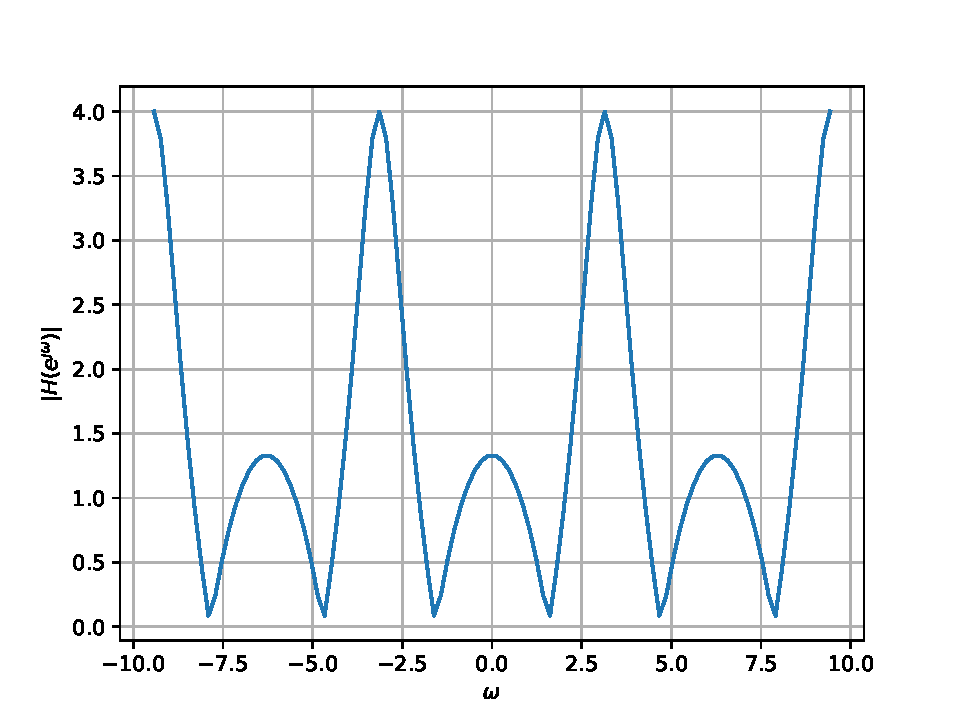
\includegraphics[width=\columnwidth]{4.5.pdf}
     \caption{$\abs{H\brak{e^{\j\omega}}}$}
     \label{fig:dtft}
\end{figure}

\item Express $h(n)$ in terms of $H(e^{\j\omega})$.\\
\solution We have,
\begin{align}
	H(e^{\j\omega}) &= \sum_{k = -\infty}^{\infty}h(k)e^{-\j\omega k}
\end{align} 
on multiplying $e^{\j\omega n}d\omega$ on both sides\\
\begin{align}
	\implies H(e^{\j\omega})e^{\j\omega n}d\omega &= \sum_{k = -\infty}^{\infty}h(k)e^{-\j\omega k}e^{\j\omega n}d\omega
\end{align} 
Now integrating on both sides from $-\pi$ to $\pi$\\
However,
\begin{align}
	\int_{-\pi}^{\pi}e^{\j\omega(n - k)}d\omega =
	\begin{cases}
		2\pi & n = k \\
		0 & \textrm{otherwise}
	\end{cases}
\end{align}
and so,
\begin{align}
	&\frac{1}{2\pi}\int_{-\pi}^{\pi}H(e^{\j\omega})e^{j\omega n}d\omega \\
	&= \frac{1}{2\pi}\sum_{k = -\infty}^{\infty}\int_{-\pi}^{\pi}h(k)e^{\j\omega(n - k)}d\omega \\
	&= \frac{1}{2\pi}2\pi h(n) = h(n)
\end{align}
 Thus,
\begin{align}
	h(n) &= \frac{1}{2\pi}\int_{-\pi}^{\pi}H(e^{\j\omega})e^{\j\omega n}d\omega \\
	\label{eq:idtft}
\end{align}
\end{enumerate}
\section{Impulse Response}
\begin{enumerate}[label=\thesection.\arabic*]
	\item Using long division, 
find $h(n)$,  $n < 5$ for H(z) in 
		\eqref{eq:freq_resp}.\\
\solution From \eqref{eq:freq_resp}, we have\\
\begin{align}
H(z) = \frac{1 + z^{-2}}{1 + \frac{1}{2}z^{-1}}
\end{align}
Substitute $z^{-1} = x$ to perform long division
\polylongdiv{1 + x^2}{1 + \frac{1}{2}x}\\

From above division we can write,
\begin{align}
1+z^{-2} &= (1+\frac{1}{2}z^{-1})(2z^{-1}-4) + 5\\
\frac{1+z^{-2}}{1+\frac{1}{2}z^{-1}} &= 2z^{-1}-4 + \frac{5}{1+\frac{1}{2}z^{-1}}
\end{align}
From \eqref{eq:freq_resp}, we can write
\begin{align}
H(z) &= -4 + 2z^{-1} + \frac{5}{1 + \frac{1}{2}z^{-1}} \\
&= -4 + 2z^{-1} + 5\sum_{n = 0}^{\infty}\brak{-\frac{1}{2}}^nz^{-n} \\
&= 1 - \frac{1}{2}z^{-1} + 5\sum_{n = 2}^{\infty}\brak{-\frac{1}{2}}^nz^{-n} \\
&= \sum_{n = 0}^{\infty}\brak{-\frac{1}{2}}^nz^{-n} + 4\sum_{n = 2}^{\infty}\brak{-\frac{1}{2}}^nz^{-n} \\
&= \sum_{n = -\infty}^{\infty}u(n)\brak{-\frac{1}{2}}^nz^{-n} + \nonumber \\
&\sum_{n = -\infty}^{\infty}u(n - 2)\brak{-\frac{1}{2}}^{n - 2}z^{-n}
\end{align}
Therefore, from \eqref{eq:z_trans}, 
\begin{align}
	h(n) = \brak{-\frac{1}{2}}^{n}u(n) + \brak{-\frac{1}{2}}^{n-2}u(n-2)
\end{align}
\item \label{prob:impulse_resp}
Find an expression for $h(n)$ using $H(z)$,\\ given that 
%in Problem \ref{eq:ztransab} and \eqref{eq:anun}, given that
\begin{equation}
\label{eq:impulse_resp}
h(n) \ztrans H(z)
\end{equation}
and there is a one to one relationship between $h(n)$ and $H(z)$.\\
$h(n)$ is known as the {\em impulse response} of the
system defined by \eqref{eq:iir_filter}.\\
\solution From \eqref{eq:freq_resp},
\begin{equation}
\label{eq:hz}
H(z) = \frac{1}{1 + \frac{1}{2}z^{-1}} + \frac{ z^{-2}}{1 + \frac{1}{2}z^{-1}}
\end{equation}
From \eqref{eq:anun},
\begin{align}
&\frac{1}{1 + \frac12 z^{-1}} \ztrans \brak{-\frac12}^n u(n) \quad \abs{z} > \frac12 \\
&\frac{z^{-2}}{1 + \frac12 z^{-1}} \ztrans \brak{-\frac12}^{n-2} u(n-2) \quad \abs{z} > \frac12\\
\Rightarrow & H(z) \ztrans \brak{-\frac12}^n u(n) + \brak{-\frac12}^{n-2} u(n-2) \quad \abs{z} > \frac12\\
\end{align}
(Since Z-transform is a linear operator)
\begin{align}
\therefore h(n) = \brak{-\frac12}^n u(n) + \brak{-\frac12}^{n-2} u(n-2) 
\end{align}
From \eqref{eq:hz},Consider the first part:
\begin{align}
\frac{1}{1 + \frac{1}{2}z^{-1}} &= \sum_{n=0}^{\infty}\brak{-\frac{1}{2}}^n z^n \quad \abs{z} > \frac12
\end{align}
and 
\begin{align}
\frac{1}{1 + \frac{1}{2}z^{-1}} &= \frac{2z}{1+2z}\\ &= \sum_{n=-\infty}^{-1}(2)^{-n}(-1)^{-n+1}z^{-n} \quad \abs{z}<\frac{1}{2}
\end{align}

Therefore, ROC of $H(z)$ will be
\begin{align}
\abs{z} \neq \frac{1}{2}
\end{align}
\item Sketch $h(n)$. Is it bounded? Convergent? \\
\solution The following code plots Fig. \ref{fig:hn}.
\begin{lstlisting}
	https://github.com/AkshithaKola/EE3900/blob/main/filter/code/5.3.py
\end{lstlisting}
and run the code using the following command
\begin{lstlisting}
python3 5.3.py
\end{lstlisting}
From the plot, we can conclude that it is convergent to 0 \\
$\therefore$ It is bounded as well.
\begin{figure}[!ht]
\centering
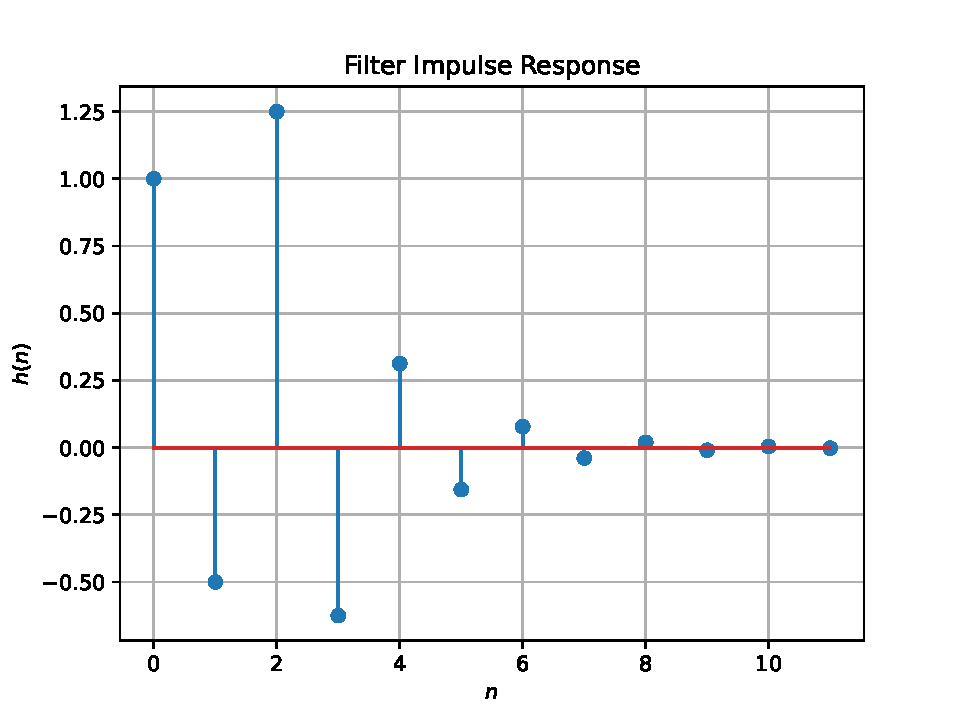
\includegraphics[width=\columnwidth]{hn.pdf}
\caption{$h(n)$ as the inverse of $H(z)$}
\label{fig:hn}
\end{figure}

\item Is it convergent? Justify using the ratio test.\\
\solution Using the ratio test for convergence
\begin{align}
\lim_{n \to \infty} \abs{\frac{h(n+1)}{h(n)}} &= \lim_{n \to \infty} \abs{\frac{\brak{-\frac{1}{2}}^{n-1} \brak{1+\frac{1}{4}}}{\brak{-\frac{1}{2}}^{n-2}\brak{1+\frac{1}{4}}}}\\ &= \lim_{n \to \infty} \abs{-\frac{1}{2}}\\ &= \frac{1}{2}<1
\end{align}
$\therefore$ h(n) is Convergent.
\item The system with $h(n)$ is defined to be stable if
\begin{equation}
\sum_{n=-\infty}^{\infty}h(n) < \infty
\end{equation}
Is the system defined by \eqref{eq:iir_filter} stable for the impulse response in \eqref{eq:impulse_resp}?\\
\solution From 5.2,
\begin{align}
\sum_{n=-\infty}^{\infty}h(n) &= \sum_{n=-\infty}^{\infty}\brak{-\frac{1}{2}}^{n}u(n) + \sum_{n=-\infty}^{\infty}\brak{-\frac{1}{2}}^{n-2}u(n-2)\\ &= \sum_{n=0}^{\infty}\brak{-\frac{1}{2}}^{n} + \sum_{n=0}^{\infty}\brak{-\frac{1}{2}}^{n-2}u(n-2)\\ &= \frac{1}{1-\brak{\frac{-1}{2}}} + \frac{1}{1-\brak{\frac{-1}{2}}}\\ &= \frac{4}{3} < \infty
\end{align}
using the fomula for the sum of an infinite geometric progression\\\\
$\therefore$ The system is stable.
\item Verify the above result using a python code.\\
\solution The following code verifies whether the given system is stable or not
\begin{lstlisting}
	https://github.com/AkshithaKola/EE3900/blob/main/filter/code/5.6.py
\end{lstlisting}
run the code using the following command
\begin{lstlisting}
python3 5.6.py
\end{lstlisting}
\item 
Compute and sketch $h(n)$ using 
\begin{equation}
\label{eq:iir_filter_h}
h(n) + \frac{1}{2}h(n-1) = \delta(n) + \delta(n-2), 
\end{equation}
%
This is the definition of $h(n)$.
\\
\solution The following code plots Fig. \ref{fig:hndef}. Note that this is the same as Fig. \ref{fig:hn}. 
%
\begin{lstlisting}
	https://github.com/AkshithaKola/EE3900/blob/main/filter/code/5.7.py
\end{lstlisting}
run the code using the following command
\begin{lstlisting}
python3 5.7.py
\end{lstlisting}
\begin{figure}[!ht]
\centering
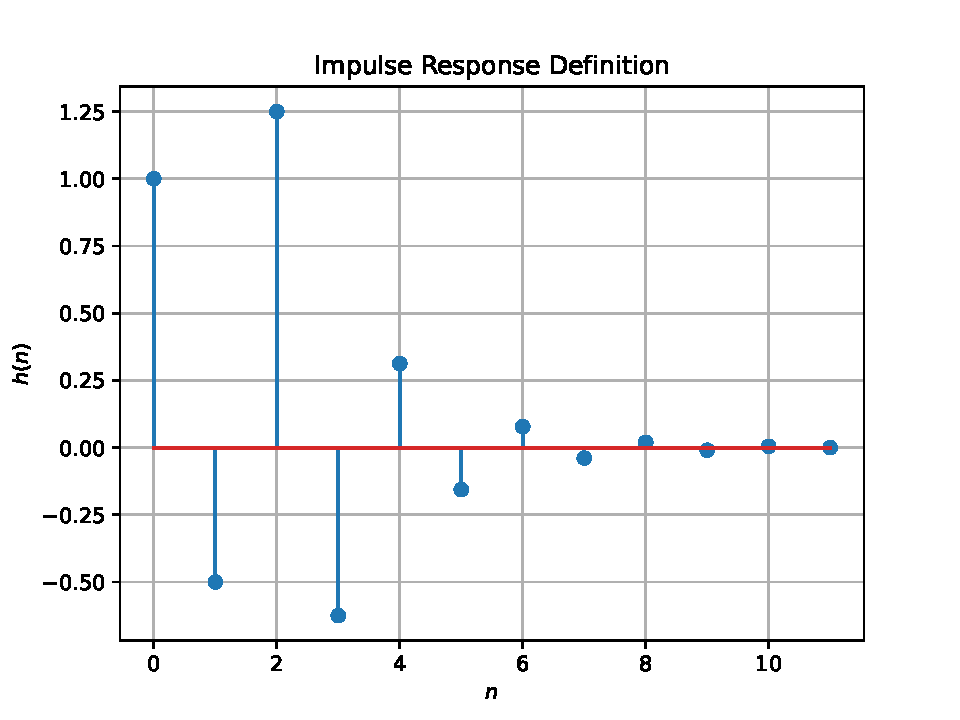
\includegraphics[width=\columnwidth]{hndef.pdf}
\caption{$h(n)$ from the definition}
\label{fig:hndef}
\end{figure}
\item Compute 
%
\begin{equation}
\label{eq:convolution}
y(n) = x(n)*h(n) = \sum_{k=-\infty}^{\infty}x(k)h(n-k)
\end{equation}
%
Comment. The operation in \eqref{eq:convolution} is known as
{\em convolution}.
%
\\
\solution 
\begin{align}
x(n)*h(n) &= \sum_{k=-\infty}^{\infty}x(k)h(n-k)\\ &= \sum_{k=0}^{5}x(k)h(n-k)
\end{align}
The following code plots Fig. \ref{fig:ynconv}.
%
\begin{lstlisting}
	https://github.com/AkshithaKola/EE3900/blob/main/filter/code/5.8.py
\end{lstlisting}
run the code using the following command
\begin{lstlisting}
python3 5.8.py
\end{lstlisting}
\begin{figure}[!htbp]
\centering
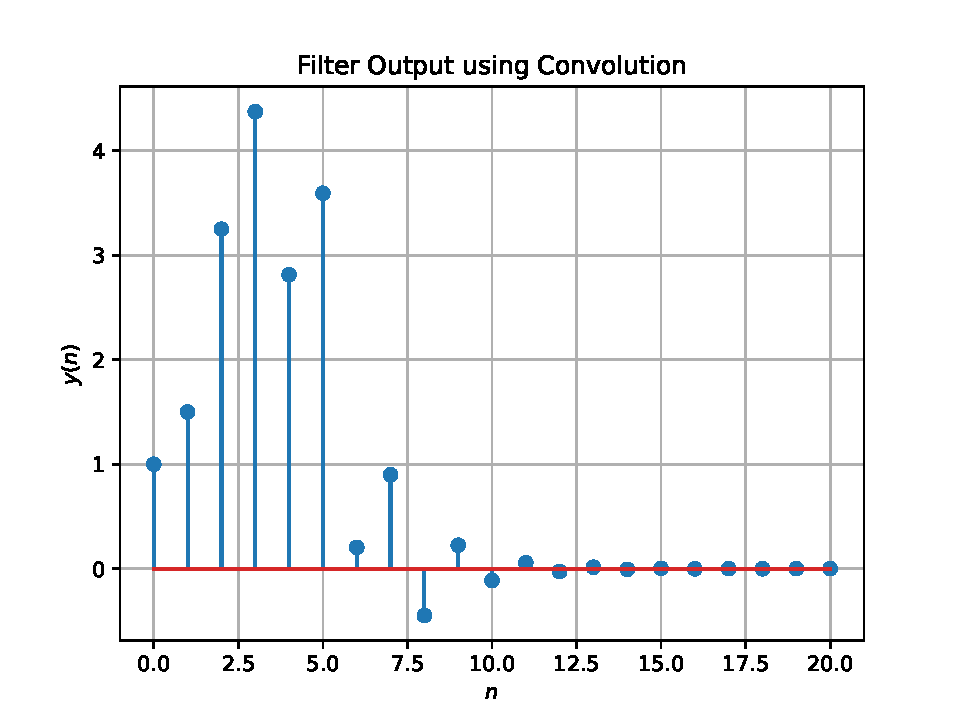
\includegraphics[width=\columnwidth]{ynconv.pdf}
\caption{$y(n)$ from the definition of convolution}
\label{fig:ynconv}
\end{figure}
This plot is same as y(n) in Fig. \ref{fig:xnyn}\\\\
Therefore,
\begin{align}
y(n) = x(n) * h(n)
\end{align}
\item Express the above convolution using a Teoplitz matrix.\\
\solution From \eqref{def:xn},we can write
\begin{align}
\vec{x} = \myvec{1 \\ 2 \\ 3 \\ 4 \\ 2 \\ 1} \qquad
\vec{h} = \myvec{1 \\ -0.5 \\ 1.25 \\ -0.62 \\ 0.31 \\ -0.16}
\end{align}
Their convolution is given by the product of the following Toeplitz matrix $\vec{T}$
\begin{align}
		&\myvec{
			1 & 0 & 0 & 0 & 0 & 0 \\
			-0.5 & 1 & 0 & 0 & 0 & 0 \\
			1.25 & -0.5 & 1 & 0 & 0 & 0 \\
			-0.62 & 1.25 & -0.5 & 1 & 0 & 0 \\
			0.31 & -0.62 & 1.25 & -0.5 & 1 & 0 \\
			-0.16 & 0.31 & -0.62 & 1.25 & -0.5 & 1 \\
			0 & -0.16 & 0.31 & -0.62 & 1.25 & -0.5 \\
			0 & 0 & -0.16 & 0.31 & -0.62 & 1.25 \\
			0 & 0 & 0 & -0.16 & 0.31 & -0.62 \\
			0 & 0 & 0 & 0 & -0.16 & 0.31 \\
			0 & 0 & 0 & 0 & 0 & -0.16 \\
		} 
\end{align}
\begin{align}
&\vec{y} = \vec{x} \circledast \vec{h} = \vec{Tx} = \myvec{1 \\ 1.5 \\ 3.25 \\ 4.38 \\ 2.81 \\ 3.59 \\ 0.12 \\ 0.78 \\ -0.62 \\ 0 \\ -0.16}
\end{align}
The following python code computes the convolution using Teoplitz matrix.
\begin{lstlisting}
	https://github.com/AkshithaKola/EE3900/blob/main/filter/code/5.9.py
\end{lstlisting}
run the code using the following command
\begin{lstlisting}
python3 5.9.py
\end{lstlisting}
\begin{figure}[!htbp]
\centering
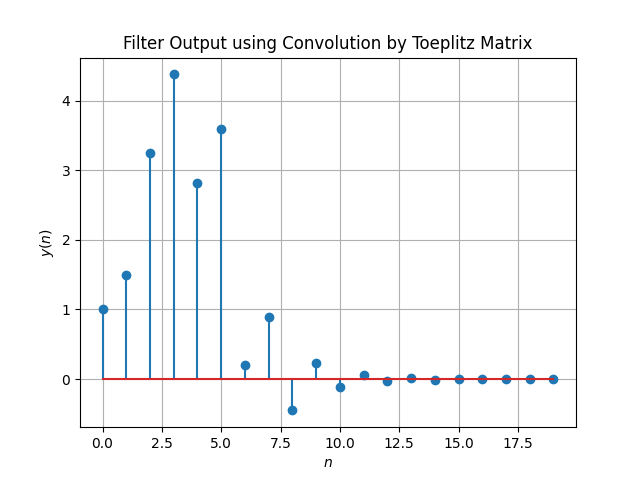
\includegraphics[width=\columnwidth]{5.9.png}
\caption{$y(n)$ from the definition of convolution using Teoplitz matrix}
\label{fig:ynconv}
\end{figure}
\item Show that
\begin{equation}
y(n) =  \sum_{k=-\infty}^{\infty}x(n-k)h(k)
\end{equation}
\solution From \eqref{eq:convolution} we know that,
\begin{align}
y(n) = x(n)*h(n) &= \sum_{k=-\infty}^{\infty}x(k)h(n-k)
\end{align}
Substitute k = n-i
\begin{align}
\sum_{k=-\infty}^{\infty}x(k)h(n-k) &= \sum_{n-i=-\infty}^{\infty}x(n-i)h(n-(n-i))\\ &= \sum_{i=\infty}^{-\infty}x(n-i)h(i)\\ &= \sum_{i=-\infty}^{\infty}x(n-i)h(i)
\end{align}
Since, the order of limit doesn't matter in case of summation.Therefore, now we have
\begin{align}
\sum_{k=-\infty}^{\infty}x(k)h(n-k) = \sum_{k=-\infty}^{\infty}x(n-k)h(k)
\end{align}
from \eqref{eq:convolution}
\begin{align}
\therefore y(n) = \sum_{k=-\infty}^{\infty}x(n-k)h(k)
\end{align}
\end{enumerate}
\section{DFT and FFT}
\begin{enumerate}[label=\thesection.\arabic*
,ref=\thesection.\theenumi]
\item
Compute
\begin{equation}
X(k) \define \sum _{n=0}^{N-1}x(n) e^{-\j2\pi kn/N}, \quad k = 0,1,\dots, N-1
\end{equation}
and $H(k)$ using $h(n)$.\\
\solution The following code plots Fig. \ref{fig:6.1}.
%
\begin{lstlisting}
	https://github.com/AkshithaKola/EE3900/blob/main/filter/code/6.1.py
\end{lstlisting}
run the above code using the command.
\begin{lstlisting}
	python3 6.1.py
\end{lstlisting}
\begin{figure}[!ht]
\centering
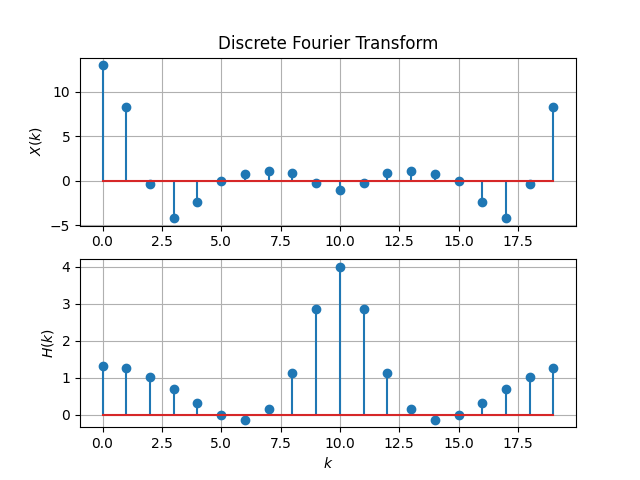
\includegraphics[width=\columnwidth]{6.1.png}
\caption{Plots of the real parts of the DFT of $x(n)$ and $h(n)$}
\label{fig:6.1}
\end{figure}
\item Compute 
\begin{equation}\label{6.2}
Y(k) = X(k)H(k)
\end{equation}
\solution Download and run the following code.
%
\begin{lstlisting}
	https://github.com/AkshithaKola/EE3900/blob/main/filter/code/6.2.py
\end{lstlisting}
run the above code using the command.
\begin{lstlisting}
	python3 6.2.py
\end{lstlisting}
\item Compute
\begin{equation} \label{6.3}
 y\brak{n}={\frac {1}{N}}\sum _{k=0}^{N-1}Y\brak{k}\cdot e^{j 2\pi kn/N},\quad n = 0,1,\dots, N-1
\end{equation}
\\
\solution The following code plots Fig. \ref{fig:ynconv}. Note that this is the same as 
$y(n)$ in  Fig. 
\ref{fig2}. 
%
\begin{lstlisting}
	https://github.com/AkshithaKola/EE3900/blob/main/filter/code/6.3.py
\end{lstlisting}
run the above code using the command.
\begin{lstlisting}
	python3 6.3.py
\end{lstlisting}
\begin{figure}[!ht]
\centering
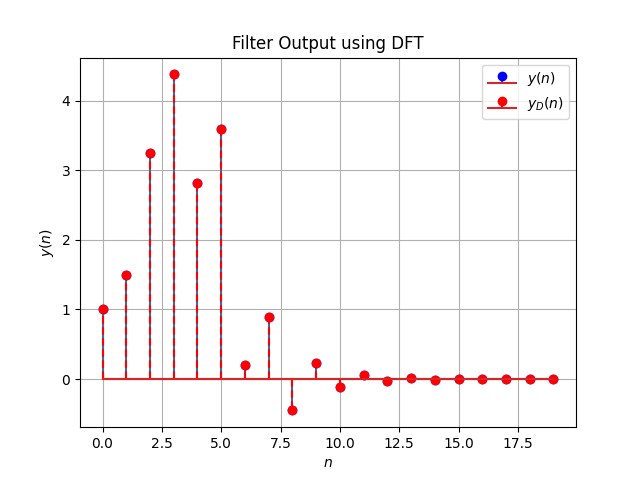
\includegraphics[width=\columnwidth]{6.3.png}
\caption{$y(n)$ from the DFT}
\label{fig:yndft}
\end{figure}
\item Repeat the previous exercise by computing $X(k), H(k)$ and $y(n)$ through FFT and 
 IFFT.
 \solution Download the code from
\begin{lstlisting}
	https://github.com/AkshithaKola/EE3900/blob/main/filter/code/6.4.py
\end{lstlisting}
and execute it using
\begin{lstlisting}
$ python3 6.4.py
\end{lstlisting}
Observe that Fig. \eqref{fig:y-n-fft} is the same as $y(n)$ in Fig. \eqref{fig2}.
\begin{figure}
\centering
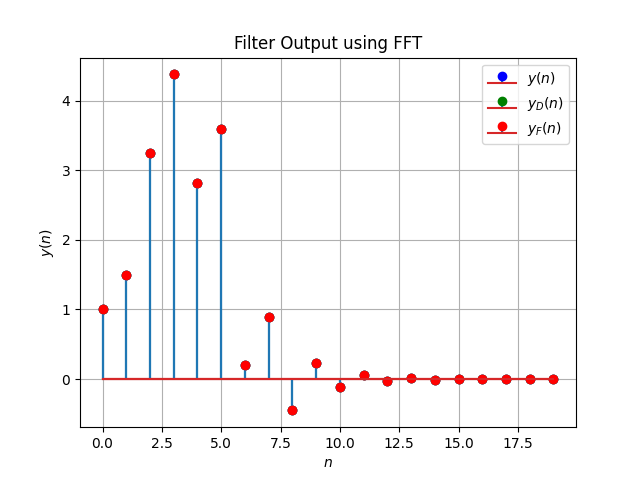
\includegraphics[width=\columnwidth]{6.4.png}
\caption{$y(n)$ using FFT and IFFT}
\label{fig:y-n-fft}
\end{figure}
\item Wherever possible, express all the above equations as matrix equations.\\
\solution
We use the DFT Matrix, where $\omega = e^{-\frac{j2k\pi}{N}}$, which is given by
\begin{align}
	\mtx{W} = 
	\begin{pmatrix}
		\omega^0 & \omega^0 & \ldots & \omega^0 \\
		\omega^0 & \omega^1 & \ldots & \omega^{N - 1} \\
		\vdots & \vdots & \ddots & \vdots \\
		\omega^0 & \omega^{N - 1} & \ldots & \omega^{(N -1)(N - 1)}
	\end{pmatrix}
\end{align}
i.e. $W_{jk} = \omega^{jk}$, $0 \leq j, k < N$. Hence, we can write any DFT equation as
\begin{align}
	\mtx{X} = \mtx{W}\mtx{x} = \mtx{x}\mtx{W}
\end{align}
\noindent where
\begin{align}
	\mtx{x} = 
	\begin{pmatrix}
		x(0) \\ x(1) \\ \vdots \\ x(n - 1)
	\end{pmatrix}
\end{align}
\noindent Using \eqref{6.3}, the inverse Fourier Transform is given by
\begin{align}
	\mtx{x} = \mathcal{F}^{-1}\brak{\mtx{X}} = \mtx{W}^{-1}\mtx{X} &= \frac{1}{N}\mtx{W^{H}}\mtx{X} = \frac{1}{N}\mtx{X}\mtx{W^{H}} \\ 
	\implies \mtx{W}^{-1} &= \frac{1}{N}\mtx{W^{H}}
\end{align}
\noindent where $H$ denotes hermitian operator. We can rewrite \eqref{6.2} using the element-wise multiplication operator as
\begin{align}
	\mtx{Y} = \mtx{H}\cdot\mtx{X} = \brak{\mtx{W}\mtx{h}}\cdot\brak{\mtx{W}\mtx{x}}
\end{align}
\item Verify the above equation by generating the DFT matrix in python.\\
\solution Download the code from
\begin{lstlisting}
	https://github.com/AkshithaKola/EE3900/blob/main/filter/code/6.6.py
\end{lstlisting}
and execute it using
\begin{lstlisting}
$ python3 6.6.py
\end{lstlisting}
The above code plots \eqref{fig:DFT matrix}
\begin{figure}
\centering
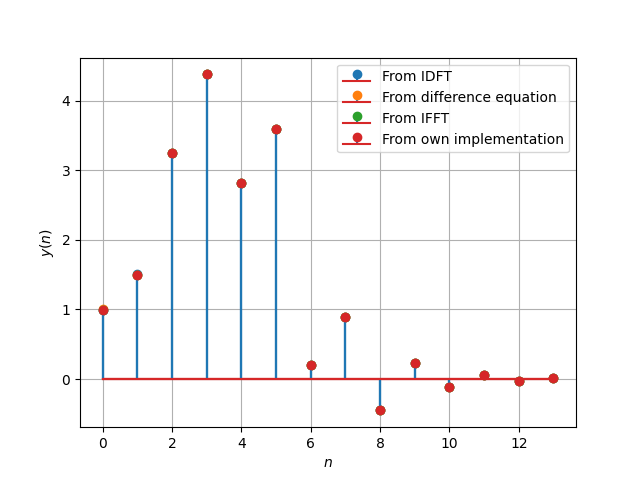
\includegraphics[width=\columnwidth]{6.6.png}
\caption{$y(n)$ using DFT matrix}
\label{fig:DFT matrix}
\end{figure}
\item Compute the 8-point FFT in C.\\
\solution Download the following C code 
\begin{lstlisting}
	https://github.com/AkshithaKola/EE3900/blob/main/filter/code/6.7.c
\end{lstlisting}
run the above C code using the command
\begin{lstlisting}
	$ gcc 6.7.c -lm -o 6.7.out
	$ ./6.7.out
\end{lstlisting}
The above code generates the text files that are loaded in the following code \\
Download the following code 
\begin{lstlisting}
	https://github.com/AkshithaKola/EE3900/blob/main/filter/code/6.7.1.py
	https://github.com/AkshithaKola/EE3900/blob/main/filter/code/6.7.2.py
\end{lstlisting}
run the above code using the command
\begin{lstlisting}
	$ python3 6.7.1_plot.py
	$ python3 6.7.2_plot.py
\end{lstlisting}
The above code plots the graphs \ref{fig:complexity fft/ifft} and \ref{fig:Complexity convolution}
\begin{figure}
\centering
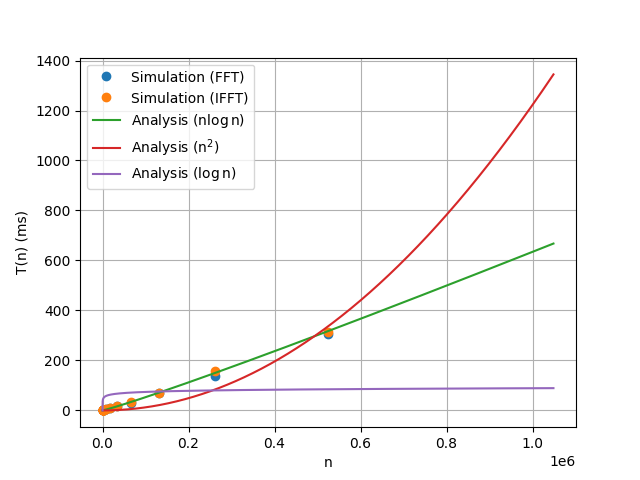
\includegraphics[width=\columnwidth]{6.7.1.png}
\caption{Complexity of FFT/IFFT is O(n log n)}
\label{fig:complexity fft/ifft}
\end{figure}
\begin{figure}
\centering
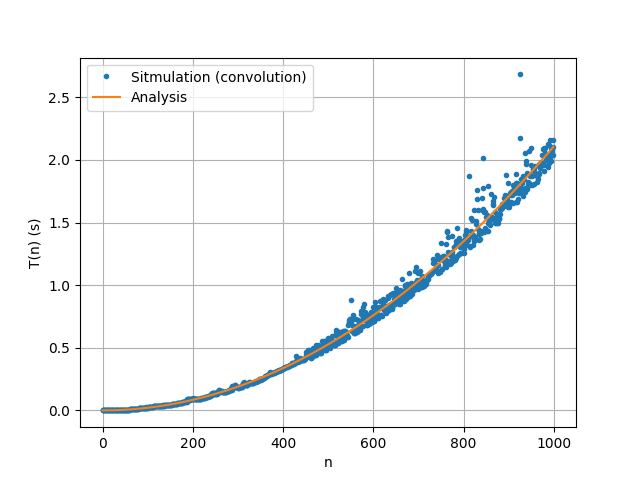
\includegraphics[width=\columnwidth]{6.7.2.png}
\caption{Complexity of convolution is O($n^2$)}
\label{fig:Complexity convolution}
\end{figure}
\end{enumerate}
\section{FFT}
 \subsection{Definitions}
\begin{enumerate}[label=\arabic*.,ref=\thesection.\theenumi]
\numberwithin{equation}{section}
    \item The DFT of $x(n)$ is given by
    \begin{align}
        X(k) \triangleq \sum_{n=0}^{N-1} x(n) e^{-j 2 \pi k n / N}, \quad k=0,1, \ldots, N-1
    \end{align}
\item Let 
	\begin{align}
W_{N} = e^{-j2\pi/N} 
	\end{align}
		Then the $N$-point {\em DFT matrix} is defined as 
	\begin{align}
		\vec{F}_{N} = \sbrak{W_{N}^{mn}}
	\end{align}
	where $W_{N}^{mn}$ are the elements of $\vec{F}_{N}$.
\item Let 
	\begin{align}
		\vec{I}_4 = \myvec{\vec{e}_4^{1} &\vec{e}_4^{2} &\vec{e}_4^{3} &\vec{e}_4^{4} }
	\end{align}
		be the $4\times 4$ identity matrix.  Then the 4 point {\em DFT permutation matrix} is defined as 
	\begin{align}
		\vec{P}_4 = \myvec{\vec{e}_4^{1} &\vec{e}_4^{3} &\vec{e}_4^{2} &\vec{e}_4^{4} }
	\end{align}
\item The 4 point {\em DFT diagonal matrix} is defined as 
	\begin{align}
		\vec{D}_4 = diag\myvec{W_{N}^{0} & W_{N}^{1} & W_{N}^{2} & W_{N}^{3}}
	\end{align}
 \end{enumerate}
 \subsection{Problems}
\begin{enumerate}[label=\arabic*.,ref=\thesection.\theenumi]
\numberwithin{equation}{section}
\item Show that 
\begin{equation} \label{wwla}
    W_{N}^{2}=W_{N/2}
\end{equation}
\solution From defination
\begin{align}
	W_{N} &= e^{-j2\pi/N} \\
	W_{N}^2 &= \brak{e^{-j2\pi/N}}^2\\
	&= e^{-j2\pi/N/2}\\
	&=W_{N/2}
\end{align}
\item Find $\vec{P}_6$.\\
\solution $\vec{P}_6 =\myvec{\vec{e}_4^{1} &\vec{e}_4^{3} &\vec{e}_4^{5} &\vec{e}_4^{2} &\vec{e}_4^{4} &\vec{e}_4^{6}}$\\
\begin{equation}
	\vec{P}_6= \myvec{&1 &0 &0 &0 &0 &0 \\&0 &0 &0 &1 &0 &0 \\&0 &1 &0 &0 &0 &0  \\&0 &0 &0 &0 &1 &0 \\&0 &0 &1 &0 &0 &0 \\&0 &0 &0 &0 &0 &1 }
\end{equation}
\item Find $\vec{D}_3$.\\
\solution \begin{align}
	\vec{D}_3 &= diag\myvec{W_{3}^{0} & W_{3}^{1} & W_{3}^{2}}\\
	& = \myvec{&1 &0 &0\\&0 &e^{-j2\pi/3} &0\\&0 &0 &(e^{-j2\pi/3})^2}
\end{align}
\item Show that 
\begin{equation}
	\vec{F}_{4}=
\begin{bmatrix}
	\vec{I}_{2} & \vec{D}_{2} \\
\vec{I}_{2} & -\vec{D}_{2}
\end{bmatrix}
\begin{bmatrix}
\vec{F}_{2} & 0 \\
0 & \vec{F}_{2}
\end{bmatrix}
\vec{P}_{4} 
\end{equation}
\solution \begin{align}
	\vec{F}_{4}\vec{P}_{4}&=
\begin{bmatrix}
	\vec{I}_{2} & \vec{D}_{2} \\
\vec{I}_{2} & -\vec{D}_{2}
\end{bmatrix}
\begin{bmatrix}
\vec{F}_{2} & 0 \\
0 & \vec{F}_{2}
\end{bmatrix}
\\
&=\begin{bmatrix}
	\vec{I}_{2}\vec{F}_{2} & \vec{D}_{2}\vec{F}_{2} \\
\vec{I}_{2}\vec{F}_{2} & -\vec{D}_{2}\vec{F}_{2}
\end{bmatrix}
\\
&= \begin{bmatrix}
	\vec{F}_{2} & \vec{D}_{2}\vec{F}_{2} \\
\vec{F}_{2} & -\vec{D}_{2}\vec{F}_{2}
\end{bmatrix}
\\
&=\begin{bmatrix}
	W_{2}^{0} &W_{2}^{0} &W_{2}^{0} &W_{2}^{0}\\
	W_{2}^{0} &W_{2}^{1} &W_{2}^{1} &W_{2}^{2}\\
	W_{2}^{0} &W_{2}^{0} &-W_{2}^{0} &-W_{2}^{0}\\
	W_{2}^{0} &W_{2}^{1} &-W_{2}^{1} &-W_{2}^{2}\\
\end{bmatrix}\\
&=\begin{bmatrix}
	1 &1 &1 &1\\
	1 &W_{2}^{1} &W_{2}^{1} &W_{2}^{2}\\
	1 &W_{2}^{0} &-W_{2}^{0} &-W_{2}^{0}\\
	1 &W_{2}^{1} &-W_{2}^{1} &-W_{2}^{2}\\
\end{bmatrix}
\end{align}
from eqn\eqref{wwla} we get $W_{2} = W_{4}^2$
\begin{align}
	\vec{F}_{4}\vec{P}_{4}&=\begin{bmatrix}
		W_{4}^{0}&W_{4}^{0}&W_{4}^{0}&W_{4}^{0}\\
		W_{4}^{0}&W_{4}^{2}&W_{4}^{1}&W_{4}^{3}\\
		W_{4}^{0}&W_{4}^{4}&W_{4}^{2}&W_{4}^{6}\\
		W_{4}^{0}&W_{4}^{6}&W_{4}^{3}&W_{4}^{9}\\
	\end{bmatrix}
\end{align}
\item Show that 
\begin{equation}
\vec{F}_{N}=
\begin{bmatrix}
\vec{I}_{N/2} & \vec{D}_{N/2} \\
\vec{I}_{N/2} & -\vec{D}_{N/2}
\end{bmatrix}
\begin{bmatrix}
\vec{F}_{N/2} & 0 \\
0 & \vec{F}_{N/2}
\end{bmatrix}
\vec{P}_{N}
\end{equation}
\solution  Observe that for even $N$ and letting $\vec{f}_N^i$ denote the $i^{\text{th}}$ column of $\vec{F}_N$, 
\begin{align}
	\myvec{\vec{D}_{N/2}\vec{F}_{N/2} \\ -\vec{D}_{N/2}\vec{F}_{N/2}} = \myvec{\vec{f}_N^{2} & \vec{f}_N^{4} & \ldots & \vec{f}_N^{N}}
\end{align}
and
\begin{align}
	\myvec{\vec{I}_{N/2}\vec{F}_{N/2} \\ \vec{I}_{N/2}\vec{F}_{N/2}} = \myvec{\vec{f}_N^{1} & \vec{f}_N^{3} & \ldots & \vec{f}_N^{N - 1}}
\end{align}
Thus,
\begin{align}
	&\myvec{\vec{I}_2\vec{F}_2 & \vec{D}_2\vec{F}_2 \\ \vec{I}_2\vec{F}_2 & -\vec{D}_2\vec{F}_2} = \myvec{\vec{I}_{N/2} & \vec{D}_{N/2} \\ \vec{I}_{N/2} & -\vec{D}_{N/2}}\myvec{\vec{F}_{N/2} & 0 \\ 0 & \vec{F}_{N/2}} \nonumber \\
	&= \myvec{\vec{f}_N^{1} & \ldots & \vec{f}_N^{N - 1} & \vec{f}_N^{2} & \ldots & \vec{f}_N^{N}}
\end{align}
and so,
\begin{align}
	&\myvec{\vec{I}_{N/2} & \vec{D}_{N/2} \\ \vec{I}_{N/2} & -\vec{D}_{N/2}}\myvec{\vec{F}_{N/2} & 0 \\ 0 & \vec{F}_{N/2}}\vec{P}_{N} \nonumber \\
	&= \myvec{\vec{f}_N^{1} & \vec{f}_N^{2} & \ldots & \vec{f}_N^{N}} = \vec{F}_N
\end{align}
\item Find 
    \begin{align}
	     \vec{P}_4 \vec{x}
    \end{align}
\solution  We have,
\begin{align}
	\vec{P}_4\vec{x} = \myvec{\vec{e}_4^1 & \vec{e}_4^3 & \vec{e}_4^2 & \vec{e}_4^4}\myvec{x(0)\\x(1)\\x(2)\\x(3)} = \myvec{x(0)\\x(2)\\x(1)\\x(3)}
	\label{eq:x-permute}
\end{align}
\item Show that 
    \begin{align}
	    \vec{X} = \vec{F}_N \vec{x}
	    \label{eq:dft-mat-def}
    \end{align}
		where $\vec{x}, \vec{X}$ are the vector representations of $x(n), X(k)$ respectively.\\
		\solution  Writing the terms of $X$, 
		\begin{align}
			X(0) &= x(0) + x(1) + \ldots + x(N - 1) \\
			X(1) &= x(0) + x(1)e^{-\frac{\j2\pi}{N}} + \ldots + \nonumber \\
				 &+ x(N - 1)e^{-\frac{\j2(N - 1)\pi}{N}} \\
				 &\vdots \nonumber \\
			X(N - 1) &= x(0) + x(1)e^{-\frac{\j2(N - 1)\pi}{N}} + \ldots + \nonumber \\
					 &+ x(N - 1)e^{-\frac{\j2(N - 1)(N - 1)\pi}{N}}	
		\end{align}
		Clearly, the term in the $m^{\text{th}}$ row and $n^{\text{th}}$ column is given by ($0 \leq m \leq N - 1$ and $0 \leq n \leq N - 1$) 
		\begin{align}
			T_{mn} = x(n)e^{-\frac{\j2mn\pi}{N}} 
		\end{align}
		and so, we can represent each of these terms as a matrix product
		\begin{align}
			\vec{X} = \vec{F}_N\vec{x}
		\end{align}
		where $\vec{F}_N = \sbrak{e^{-\frac{-\j2mn\pi}{N}}}_{mn}$ for $0 \leq m \leq N - 1$ and $0 \leq n \leq N - 1$.
\item Derive the following Step-by-step visualisation  of
8-point FFTs into 4-point FFTs and so on
\begin{equation}
\begin{bmatrix}
X(0) \\ 
X(1) \\ 
X(2) \\ 
X(3)
\end{bmatrix}
=
\begin{bmatrix}
X_{1}(0) \\ 
X_{1}(1)\\ 
X_{1}(2)\\
X_{1}(3)\\
\end{bmatrix}
+
\begin{bmatrix}
W^{0}_{8} & 0 & 0 & 0\\
0 & W^{1}_{8} & 0 & 0\\
0 & 0 & W^{2}_{8} & 0\\
0 & 0 & 0 & W^{3}_{8}
\end{bmatrix}
\begin{bmatrix}
X_{2}(0) \\ 
X_{2}(1) \\ 
X_{2}(2) \\
X_{2}(3)
\end{bmatrix}
\end{equation}
\begin{equation}
\begin{bmatrix}
X(4) \\ 
X(5) \\ 
X(6) \\ 
X(7)
\end{bmatrix}
=
\begin{bmatrix}
X_{1}(0) \\ 
X_{1}(1)\\ 
X_{1}(2)\\
X_{1}(3)\\
\end{bmatrix}
-
\begin{bmatrix}
W^{0}_{8} & 0 & 0 & 0\\
0 & W^{1}_{8} & 0 & 0\\
0 & 0 & W^{2}_{8} & 0\\
0 & 0 & 0 & W^{3}_{8}
\end{bmatrix}
\begin{bmatrix}
X_{2}(0) \\ 
X_{2}(1) \\ 
X_{2}(2) \\
X_{2}(3)
\end{bmatrix}
\end{equation}
4-point FFTs into 2-point FFTs
\begin{equation}
\begin{bmatrix}
X_{1}(0) \\ 
X_{1}(1)\\ 
\end{bmatrix}
=
\begin{bmatrix}
X_{3}(0) \\ 
X_{3}(1)\\ 
\end{bmatrix}
+
\begin{bmatrix}
W^{0}_{4} & 0\\
0 & W^{1}_{4}
\end{bmatrix}
\begin{bmatrix}
X_{4}(0) \\ 
X_{4}(1) \\ 
\end{bmatrix}
\end{equation}
\begin{equation}
\begin{bmatrix}
X_{1}(2) \\ 
X_{1}(3)\\ 
\end{bmatrix}
=
\begin{bmatrix}
X_{3}(0) \\ 
X_{3}(1)\\ 
\end{bmatrix}
-
\begin{bmatrix}
W^{0}_{4} & 0\\
0 & W^{1}_{4}
\end{bmatrix}
\begin{bmatrix}
X_{4}(0) \\ 
X_{4}(1) \\ 
\end{bmatrix}
\end{equation}
\begin{equation}
\begin{bmatrix}
X_{2}(0) \\ 
X_{2}(1)\\ 
\end{bmatrix}
=
\begin{bmatrix}
X_{5}(0) \\ 
X_{5}(1)\\ 
\end{bmatrix}
+
\begin{bmatrix}
W^{0}_{4} & 0\\
0 & W^{1}_{4}
\end{bmatrix}
\begin{bmatrix}
X_{6}(0) \\ 
X_{6}(1) \\ 
\end{bmatrix}
\end{equation}
\begin{equation}
\begin{bmatrix}
X_{2}(2) \\ 
X_{2}(3)\\ 
\end{bmatrix}
=
\begin{bmatrix}
X_{5}(0) \\ 
X_{5}(1)\\ 
\end{bmatrix}
-
\begin{bmatrix}
W^{0}_{4} & 0\\
0 & W^{1}_{4}
\end{bmatrix}
\begin{bmatrix}
X_{6}(0) \\ 
X_{6}(1) \\ 
\end{bmatrix}
\end{equation}
\begin{equation}
P_{8}
\begin{bmatrix}
x(0) \\ 
x(1) \\ 
x(2) \\ 
x(3) \\ 
x(4) \\ 
x(5) \\
x(6) \\
x(7)
\end{bmatrix}
 = 
\begin{bmatrix}
x(0) \\ 
x(2) \\ 
x(4) \\ 
x(6) \\
x(1) \\ 
x(3) \\ 
x(5) \\
x(7)
\end{bmatrix}
\end{equation}
\begin{equation}
P_{4}
\begin{bmatrix}
x(0) \\ 
x(2) \\ 
x(4) \\ 
x(6) \\
\end{bmatrix}
 = 
\begin{bmatrix}
x(0) \\ 
x(4) \\ 
x(2) \\
x(6)
\end{bmatrix}
\end{equation}
\begin{equation}
P_{4}
\begin{bmatrix}
x(1) \\ 
x(3) \\ 
x(5) \\
x(7)
\end{bmatrix}
 = 
\begin{bmatrix}
x(1) \\ 
x(5) \\ 
x(3) \\ 
x(7) \\
\end{bmatrix}
\end{equation}
Therefore,
\begin{equation}
\begin{bmatrix}
X_{3}(0) \\ 
X_{3}(1)\\ 
\end{bmatrix}
= F_{2}
\begin{bmatrix}
x(0) \\ 
x(4) \\ 
\end{bmatrix}
\end{equation}
\begin{equation}
\begin{bmatrix}
X_{4}(0) \\ 
X_{4}(1)\\ 
\end{bmatrix}
= F_{2}
\begin{bmatrix}
x(2) \\ 
x(6) \\ 
\end{bmatrix}
\end{equation}
\begin{equation}
\begin{bmatrix}
X_{5}(0) \\ 
X_{5}(1)\\ 
\end{bmatrix}
= F_{2}
\begin{bmatrix}
x(1) \\ 
x(5) \\ 
\end{bmatrix}
\end{equation}
\begin{equation}
\begin{bmatrix}
X_{6}(0) \\ 
X_{6}(1)\\ 
\end{bmatrix}
= F_{2}
\begin{bmatrix}
x(3) \\ 
x(7) \\ 
\end{bmatrix}
\end{equation}
\item For 
    \begin{align}
	    \vec{x} = \myvec{1\\2\\3\\4\\2\\1}
        \label{eq:equation1}
    \end{align}
    compte the DFT  
		using 
	    \eqref{eq:dft-mat-def}\\
\solution Download the code from
\begin{lstlisting}
	https://github.com/AkshithaKola/EE3900/blob/main/filter/code/7.9.py
\end{lstlisting}
and execute it using
\begin{lstlisting}
$ python3 7.9.py
\end{lstlisting}
\item Repeat the above exercise using the FFT
after zero padding $\vec{x}$.\\
\solution Download the code from
\begin{lstlisting}
	https://github.com/AkshithaKola/EE3900/blob/main/filter/code/7.10.py
\end{lstlisting}
and execute it using
\begin{lstlisting}
$ python3 7.10.py
\end{lstlisting}
\item Write a C program to compute the 8-point FFT.\\
\solution Download the code from
\begin{lstlisting}
	https://github.com/AkshithaKola/EE3900/blob/main/filter/code/7.11.c
\end{lstlisting}
compile it using
\begin{lstlisting}
$ gcc 7.11.c -lm 
\end{lstlisting}
and execute it using
\begin{lstlisting}
$ ./a.out
\end{lstlisting}
 \end{enumerate}

\end{document}